\section{Timeplan}

\subsection{Time Management Towards the Deadline}

After the project kick-off at the beginning of February, the team intends on spending the entire month in the planning phase. We think
this is the right decision as it will allow us to carefully examine each aspect of our project, from the business standpoint, the requirements
and component structure to the security, release planning and post-launch maintenance. Such a time window will allow us to carry out a design sprint or
a \hyperref[sec:MiniSprint]{mini design sprint}, documents from which were described in 
the \hyperref[sec:UserJourneyMaps]{Analysis}, as well as prepare the following items before we can start the development stage:
\begin{itemize}
    \item Figma Prototype, see \hyperref[sec:Design]{Design}
    \item UML Component Diagram
    \item UML Context Diagram
    \item Excel Spreadsheet with Project Requirements, Time Estimations and MoSCoW Prioritization
    \item UML Data Model Diagram
    \item UML Class Diagram
    \item Business Model, along with Personas and Value Proposition Canvases
    \item UML Use Case Diagrams
    \item UML Sequence Diagrams
    \item UML State Machine Diagrams
\end{itemize}

Once the initial documentation phase is finished, the team will move onto the development phase which will last until the beginning
of May and will result in the delivery of the Minimum Viable Product for LinkedGym. Next, the team will spend the rest of May adding more features and polishing
the product to be ready for the realease of the Minimum Marketable Product at the beginning of June. At this point, the team will continue on adding features 
that have been prioritized as "Could", implementing user feedback and fixing any bugs that will pop up, but the project will move into the final, maintenance phase.

\begin{figure}[H]
    \centering
    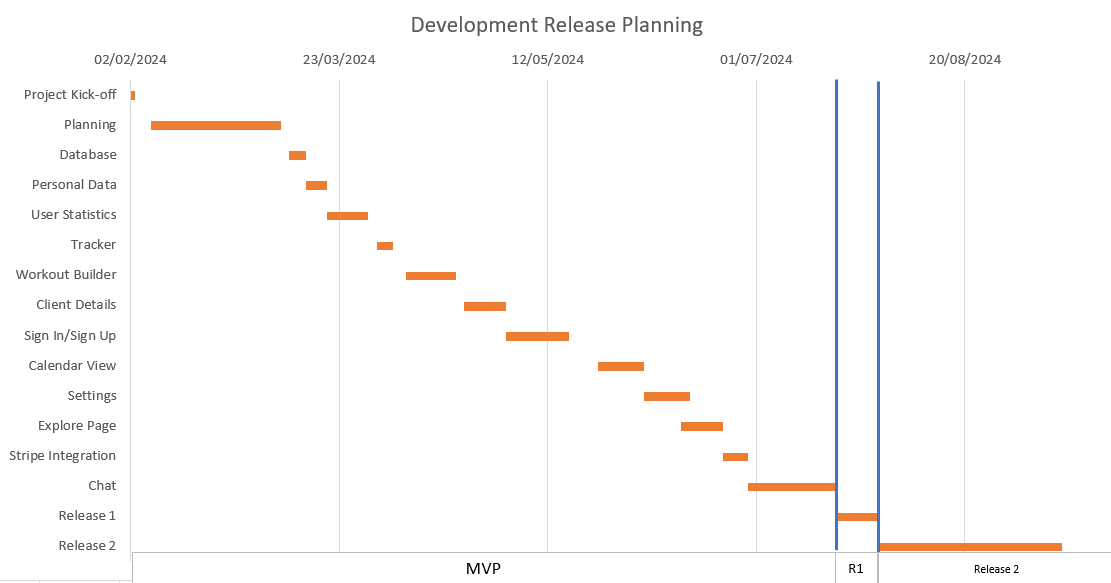
\includegraphics[width=0.8\textwidth]{images/initial_gantt_chart.png}
    \caption{First Version of the Timeplan Gantt Chart}
    \label{fig:initialganttchart}
\end{figure}

\begin{figure}[H]
    \centering
    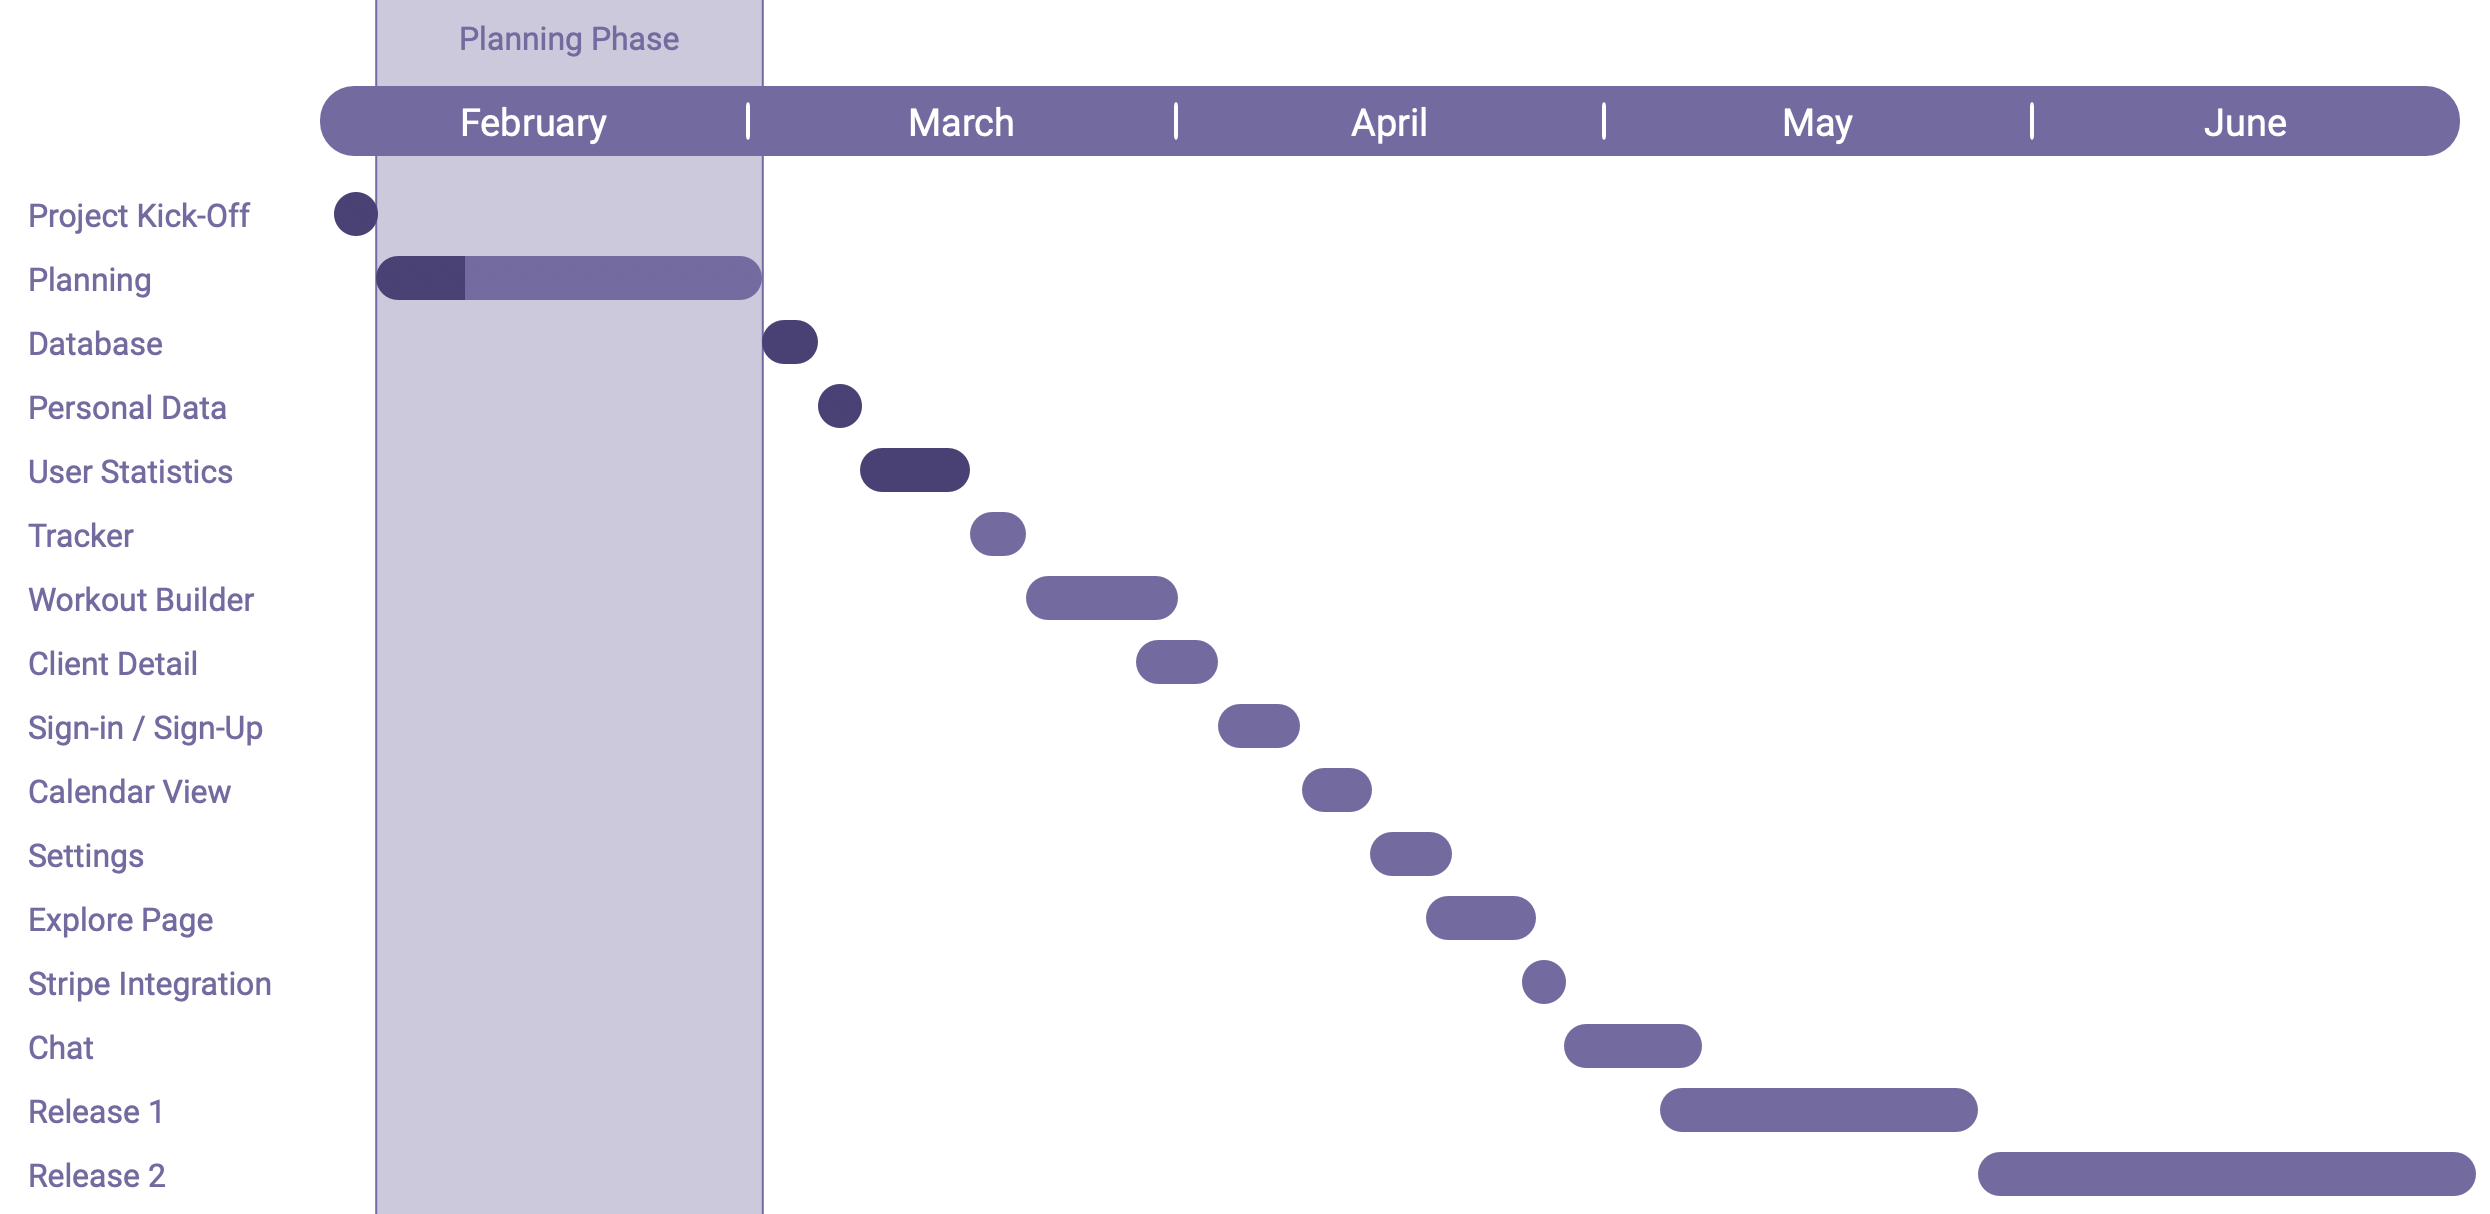
\includegraphics[width=0.8\textwidth]{images/gantt_chart.png}
    \caption{Second Version of the Timeplan Gantt Chart}
    \label{fig:ganttchart}
\end{figure}

\subsection{Time Estimates}
To prepare a Time Management plan as seen in the previous section, the team has conducted both a top-down, as well as a bottom-up 
time estimation for each requirement, to ensure our resutls are as accurate as possible. We went through this process twice during the
project, as we were not happy with the initial estimates we got. In the end, we are confident in our plan. We followed the requirement
structure from the \hyperref[sec:Requirements]{Requirements Chapter}.
For the estimation process we used a Microsoft Excel Workbook, where each Spreadsheet corresponded to one component, and contained
all of it's requirements. As our estimation factor, we chose to use the number pi rounded up to two decimal places - 3,14. We also chose to
use MoSCoW prioritization for each requirement. The result of our work can be seen below in the attached print out of the spreadsheets.

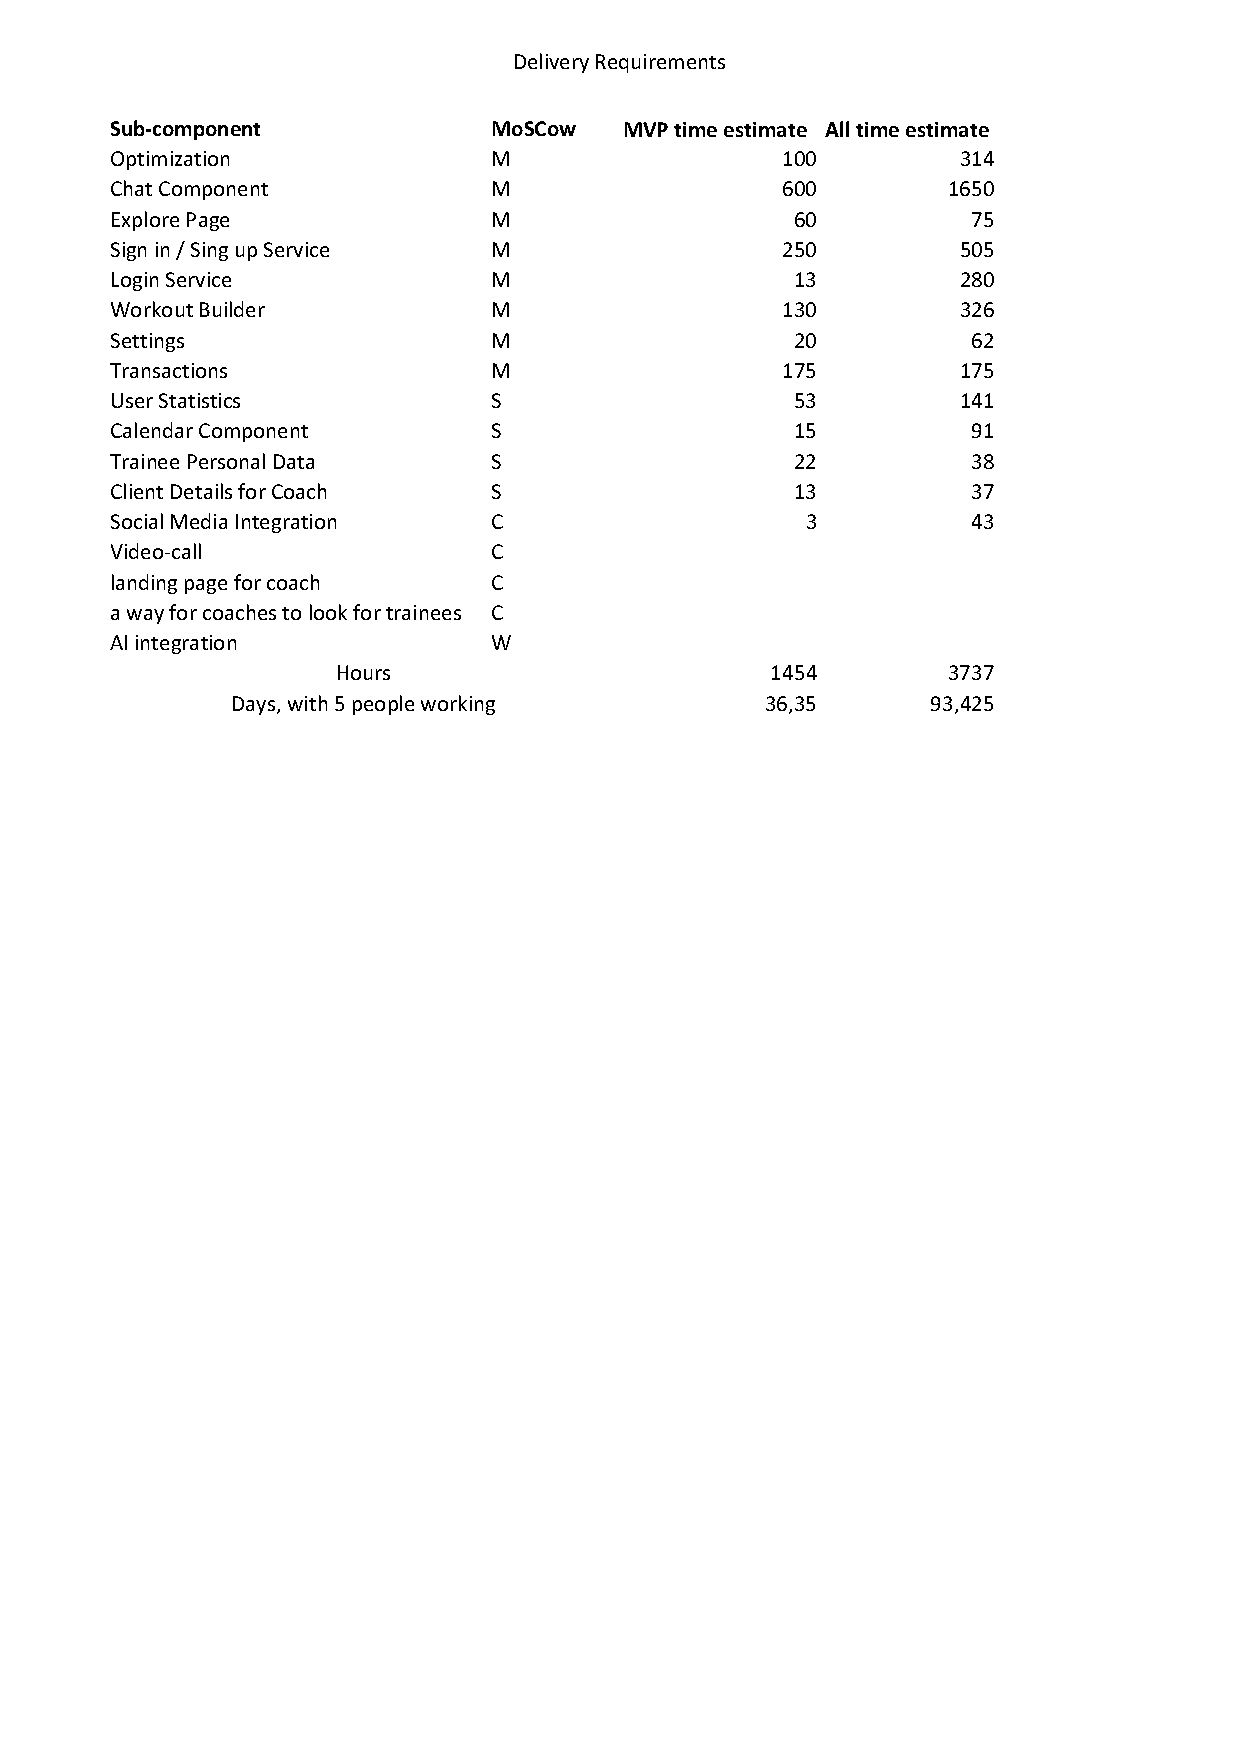
\includepdf[pages=-]{Resources/LinkedGym_requirements_estimates_prio.pdf}

\subsection{How the methodology affects our timeplan}
As we mentioned in the \hyperref[sec:Methodology]{Methodology Chapter}, our methodology of choice is Agile applied in the Scrum framework.
It was one of the greatest factors we took into account when creating our timeplan, making sure the project applies Agile principles,
and follows the structure of Scrum. That is how we ended up with a shorter planning phase followed by a long development phase, during which
we have the freedom of adjusting and creating more documentation as needed. Another result of our framework choice is our release plan,
which consists of, most notably, the MVP and MMP releases. We also planned for releases after the MMP, to allign with Scrum's premise
of meeting customer expectations and incrementing on the product.
Scrum events were also an important factor to consider during time estimation, since, on average, they take out one working day from 
a full workweek. We tried to account for this setback in time in our charts as best as we could, by manually adjusting margins and
counting Scrum events into our time estimates.

\subsection{Strategy for Project Completion and Sprint Setup}
To ensure the project completion we would stick closely to our chosen methodology and framework;
\begin{itemize}
    \item We would divide ourselves into the Scrum Team: Product Owner, Scrum Master and Development Team
    \item Throughout the development phase we would conduct Sprints that would increment on the product, check of items from the backlog, and last 2-4 weeks
    \item Before each sprint, we would appoint one day to sprint planning, to define a goal for the sprint for our stakeholders and appoint items from the product backlog into the sprint backlog, breaking them down into more manageable tasks
    \item During each sprint, we would conduct the Daily Scrum, during which the development team would align themselves on the progress, change the status of items in the sprint backlog, make plans for the next day, validate their work with the Definition of Done and adjust as needed
    \item After each sprint, we would carry out a Sprint Review, in which we would present the done items, talk about the adjustments made during the sprint and give feedback
    \item Following the Sprint Review, a Sprint Retrospective would take place, reflecting on how the sprint went and capturing ways of increasing quality and productivity
\end{itemize}
Sticking to the Agile principles we would also pay close attention to customer satisfaction and stakeholder feedback, pivoting if necessary.

For our Sprint Setup, we would use the platform Jira in it's Scrum configuration for running our framework. The backlog is already prepared before
development begins during the Planning Phase of the project, filled out by user stories with acceptance criteria, ready to be broken
down into tasks. For source control we would use GitHub, which allows for integration with Jira, making our platforms a fully cohesive system.
Lastly, we would share our documentation and external files through Google Drive.

\subsection{Scaling agile up and down}
Since our team is not big enough to consider a scaled up Agile framework, we do not intend on scaling Scrum either up or down, instead
using the framework in it's original format throughout the development. The only point in our project which could be considered as scaling
our methodology would be moving into the maintenance phase because the frequency of the development would be lowered as the team would
move on to other projects.

Having said that, if we were to try and carry out this project in a larger team, we would have chosen to implement Large Scale Scrum (LeSS).
The reason for that choice is that it seems to us like the simplest way of applying the principles, purpose, elements, and elegance
of Scrum in a large-scale context. Simplicity is very valuable in our situation, as we have never conducted scaling agile, so starting out
with a simple method of achieving that goal seems like the most reasonable solution. The scaling up would begin shortly before the start
of the development phase, after we would have prepared our documentation. Following this, we would begin scaling down the operation as the
development phase would near its end, going back to a standard Scrum setup. The process of scaling up and down would not pose much of a challenge
as LeSS uses only a single backlog, therefore we could prepare the project just as we would do it normally, then start assigning
portions of the backlog to each team, to finally take the leftovers from the backlog when going back to Scrum.
